\documentclass[11pt,reqno]{amsart}

% --- Encoding / fonts ---
\usepackage[T1]{fontenc}
\usepackage[utf8]{inputenc}

% --- Core AMS packages ---
\usepackage{amsmath,amssymb,amsfonts,amsthm,mathtools}

% --- Graphics and lists ---
\usepackage{graphicx}
\usepackage{enumitem}

% --- Page layout ---
\usepackage[a4paper,margin=3cm]{geometry}

% --- Theorem environments ---
\theoremstyle{plain}
\newtheorem{theorem}{Theorem}[section]
\newtheorem{lemma}[theorem]{Lemma}
\newtheorem{proposition}[theorem]{Proposition}
\newtheorem{corollary}[theorem]{Corollary}

\theoremstyle{definition}
\newtheorem{definition}[theorem]{Definition}
\newtheorem{example}[theorem]{Example}
\newtheorem{question}[theorem]{Question}
\newtheorem{conjecture}[theorem]{Conjecture}

\theoremstyle{remark}
\newtheorem{remark}[theorem]{Remark}
\newtheorem{claim}[theorem]{Claim}
\newtheorem{assertion}[theorem]{Assertion}
\newtheorem{notations}[theorem]{Notations}

\newtheorem{assumption}{Assumption}
\newtheorem{hypothesis}{Hypothesis}

\newtheorem*{theoremA}{Theorem A}
\newtheorem*{theoremB}{Theorem B}
\newtheorem*{theoremC}{Theorem C}

% --- Operators ---
\DeclareMathOperator{\IFS}{IFS}
\DeclareMathOperator{\diam}{diam}
\DeclareMathOperator{\vol}{vol}

% --- Hyperref: load late ---
\usepackage[pdfencoding=auto,psdextra]{hyperref}

% --- TOC depth ---
\setcounter{tocdepth}{3}

% --- Title & Authors ---
\title[T]{TransTitle}

\author[A1]{B1}
\address{Department of Pure Mathematics, Ferdowsi University of Mashhad, Mashhad, Iran}
\email{htina@um.ac.ir}

\author[A2]{B2}
\address{Department of Pure Mathematics, Ferdowsi University of Mashhad, Mashhad, Iran}
\email{zaj@ferdowsi.um.ac.ir}

\thanks{Corresponding author: F. H. Ghane (\texttt{htina@um.ac.ir})}

\keywords{Monotone}
\subjclass[2020]{Primary 37D25; Secondary 37A35, 37C40, 37A60.}

\begin{document}

\maketitle


\begin{abstract}
aaaaaaaaa
\end{abstract}

\section{Introduction}
\label{sec:intro}

\section{The Simplified Model}

The general 2D Hindmarsh--Rose-type system is given by:
\begin{equation}
\begin{aligned}
\dot{x} &= y - ax^3 + bx^2 + I, \\
\dot{y} &= c - dx^2 - y,
\end{aligned}
\end{equation}
where \(x\) represents the membrane potential, \(y\) is the recovery variable, and \(I\) is the external input current. The parameters \(a, b, c, d\) control the intrinsic nonlinearities.

To obtain a mathematically tractable model for global phase-portrait analysis, we fix the parameters as follows:
\begin{itemize}
    \item \(a = 1\)
    \item \(c = 1\)
    \item \(b = d = k\) (where \(k\) is a fixed positive constant, biologically motivated by the standard Hindmarsh--Rose baseline \(k=5\))
\end{itemize}

The system reduces to:
\begin{equation}
\label{eq:model}
\begin{cases}
\dot{x}=y-x^3+kx^2+I,\\[1mm]
\dot{y}=1-kx^2-y,
\end{cases}
\end{equation}
where, \(I\) and $k$ are parameters of system.

\section{Hopf Bifurcation and Preliminary Analysis of Limit Cycles}

We consider the following planar system
\eqref{eq:model}. The aim of this section is to
investigate the occurrence of Hopf bifurcation and derive a suitable
formulation for the study of periodic solutions.

\subsection{The equilibrium point and Hopf bifurcation}

The equilibrium points of system \eqref{eq:model} satisfy
\[
y-x^3+kx^2+I=0,
\]
and
\[
1-kx^2-y=0.
\]
Hence system \eqref{eq:model} has a unique equilibrium point
\begin{equation}
\label{eq:equilibrium}
E_*=(x_*,y_*),
\end{equation}
where
\begin{equation*}
\label{eq:xstar}
x_*=(1+I)^{1/3},
\end{equation}
and
\begin{equation*}
\label{eq:ystar}
y_*=1-kx_*^2 .
\end{equation}
The Jacobian matrix of system \eqref{eq:model} is
\[
J(x,y)=
\begin{pmatrix}
-3x^2+2kx&1\\
-2kx&-1
\end{pmatrix}.
\]
At the equilibrium point $E_*$ we have
\[
J(E_*)=
\begin{pmatrix}
-3x_*^2+2kx_*&1\\
-2kx_*&-1
\end{pmatrix}.
\]
The trace and determinant of this matrix are
\begin{equation}
\label{eq:trace}
T=-3x_*^2+2kx_*-1,
\end{equation}
and
\begin{equation}
\label{eq:det}
D=
(-3x_*^2+2kx_*)(-1)+2kx_*.
\end{equation}
Therefore,
$
D=3x_*^2.
$

The necessary conditions for a Hopf bifurcation are
\[
T=0,\qquad D>0.
\]
The trace condition gives
$
-3x_*^2+2kx_*-1=0,
$
and therefore the Hopf curve is
\begin{equation}
\label{eq:Hopfcurve}
k=k_H=
\frac{3x_*^2+1}{2x_*}.
\end{equation}
And
$
D=3x_*^2>0,
$
and
$
x_*\neq0,
$
or equivalently,
$
I\neq -1.
$

So, at the Hopf point, the eigenvalues of $J(E_*)$ are
\[
\lambda_{1,2}=\pm i\omega,
\]
where
\begin{equation}
\label{eq:omega}
\omega=\sqrt{3}|x_*|.
\end{equation}
It remains to verify the transversality condition. By \eqref{eq:trace}
we obtain
$
\frac{dT}{dk}=2x_*.
$
Because
$
\operatorname{Re}(\lambda)=\frac{T}{2},
$
we have
\[
\frac{d}{dk}\operatorname{Re}(\lambda)
=
x_*.
\]
Therefore,

\[
\frac{d}{dk}\operatorname{Re}(\lambda)
\neq0
\]

whenever $I\neq-1$. Consequently, system \eqref{eq:model}
undergoes a Hopf bifurcation on the curve \eqref{eq:Hopfcurve}.


\subsection{The first Lyapunov coefficient}

To determine the type of Hopf bifurcation, we translate the equilibrium
point $E_*$ to the origin by introducing
\[
x=x_*+u,\qquad y=y_*+v .
\]
Then system \eqref{eq:model} becomes
\begin{equation}
\label{eq:shifted}
\begin{cases}
\dot{u}=(-3x_*^2+2kx_*)u+v
 +(k-3x_*)u^2-u^3,\\[1mm]
\dot{v}=-2kx_*u-v-ku^2 .
\end{cases}
\end{equation}
At the Hopf point $k=k_H$, using
$
2k_Hx_*=3x_*^2+1,
$
the linear part of \eqref{eq:shifted} is
\[
A=
\begin{pmatrix}
1&1\\
-(3x_*^2+1)&-1
\end{pmatrix}.
\]
The nonlinear terms are
\[
F_2(u,v)=
\begin{pmatrix}
(k_H-3x_*)u^2\\
-k_Hu^2
\end{pmatrix},
\]
and
\[
F_3(u,v)=
\begin{pmatrix}
-u^3\\
0
\end{pmatrix}.
\]
Using the standard formula for the first Lyapunov coefficient of a
planar Hopf bifurcation, after substituting the eigenvectors of $A$ and
simplifying the resulting expression, we obtain

\begin{equation}
\label{eq:l1}
l_1=
-\frac{3x_*^2+1}
{8\sqrt{3}\,x_*^2}.
\end{equation}
Since
$
3x_*^2+1>0,
$
we conclude that
$
l_1<0 .
$
Hence the Hopf bifurcation is supercritical and a stable limit cycle
bifurcates from the equilibrium point when the parameter crosses the
Hopf curve.
Thus, we have theorem:
\begin{theorem}
\label{thm:hopf_limit_cycle}
Consider the planar system
\eqref{eq:model}
where $k$ and $I$ are real parameters. Let
$
x_*=(1+I)^{1/3},
$
and assume that
$
I\neq -1.
$
Then this system has a unique equilibrium point
\[
E_*=
\left(
x_*,
1-kx_*^2
\right).
\]
Moreover, the equilibrium undergoes a supercritical Hopf bifurcation at the
parameter value
$k=k_H$
\eqref{eq:Hopfcurve}.
 Hence, for
parameter values sufficiently close to and beyond the Hopf curve,
system \eqref{eq:model} possesses a stable limit cycle bifurcating
from the equilibrium point $E_*$.
\end{theorem}

%\begin{proof}
%The equilibrium point is obtained by solving
%\[
%y-x^3+kx^2+I=0,
%\qquad
%1-kx^2-y=0,
%\]
%which gives
%\[
%x_*^3=1+I,
%\qquad
%y_*=1-kx_*^2.
%\]
%The Jacobian matrix is
%\[
%J(x,y)=
%\begin{pmatrix}
%-3x^2+2kx&1\\
%-2kx&-1
%\end{pmatrix}.
%\]
%Therefore, at $E_*$,
%\[
%\operatorname{tr}(J)
%=-3x_*^2+2kx_*-1, \]
%and
%\[ \det(J)=3x_*^2. \]
%\The Hopf condition
%\[
%\operatorname{tr}(J)=0\]
%gives
%\[
%k_H=\frac{3x_*^2+1}{2x_*}.
%\]
%Since $I\neq-1$, we have $x_*\neq0$ and hence
%\[
%\det(J)=3x_*^2>0.
%\]
%Thus the eigenvalues are purely imaginary at the Hopf point.
%Furthermore,
%\[
%\frac{d}{dk}\operatorname{Re}(\lambda)
%=
%\frac12
%\frac{d}{dk}\operatorname{tr}(J)
%%=
%x_* \neq0,
%\]
%which verifies the transversality condition.
%Finally, applying the standard formula for the first Lyapunov
%coefficient of a planar Hopf bifurcation to the translated system gives
%\[
%l_1=
%-\frac{3x_*^2+1}{8\sqrt3\,x_*^2}.
%\]
%Since $x_*\neq0$, we have $l_1<0$. Hence the Hopf bifurcation is
%supercritical and a stable periodic orbit is generated from the
%equilibrium point.
%\end{proof}

%\subsection{Trace and Determinant}
%\subsection{Classification of the Singular Point}
%\begin{itemize}
   % \item If \(T^2 - 4D > 0\): Node (stable if \(T < 0\), unstable if \(T > 0\)).
    %\item If \(T^2 - 4D < 0\): Focus (stable if \(T < 0\), unstable if \(T > 0\)).
    %\item If \(T = 0\) and \(D > 0\): Center (linearization) or weak focus.
%\end{itemize}



\subsection{Local classification of the finite equilibrium}
Since  \(D > 0\) for all \(I > -1\). Therefore, the equilibrium is never a saddle. It is either a node or a focus, and its stability is determined entirely by the sign of the trace \(T\).
Set
$
x_*=(1+I)^{1/3}>0.
$
For Hopf value \eqref{eq:Hopfcurve}
we have
\[
T=2x_*(k-k_H).
\]
and
\[
T^2-4D
=
4x_*^2\left[(k-k_H)^2-3\right].
\]
Hence the node--focus transitions occur at
\[
k_{\pm\sqrt{3}}=k_H\pm\sqrt{3}.
\]

Since
$
k_{-\sqrt{3}}
=
\frac{(\sqrt{3}\,x_*-1)^2}{2x_*}\geq0,
$
the local type of \(E_*\), for \(k>0\), is classified as follows:
\[
\begin{array}{c|c}
\text{Parameter range} & \text{Type of }E_* \\ \hline
0<k<k_H-\sqrt{3}
    & \text{hyperbolic stable node}, \\[1mm]
k=k_{-\sqrt{3}}
    & \text{stable improper node}, \\[1mm]
k_{-\sqrt{3}}<k<k_H
    & \text{hyperbolic stable focus}, \\[1mm]
k=k_H
    & \text{stable weak focus (Hopf point)}, \\[1mm]
k_H<k<k_{+\sqrt{3}}
    & \text{hyperbolic unstable focus}, \\[1mm]
k=k_{+\sqrt{3}}
    & \text{unstable improper node}, \\[1mm]
k>k_{+\sqrt{3}}
    & \text{hyperbolic unstable node}.
\end{array}
\]
Therefore, as \(k\) increases, the finite equilibrium passes through
the sequence
\[
\text{stable node}
\;\longrightarrow\;
\text{stable focus}
\;\longrightarrow\;
\text{stable weak focus}
\;\longrightarrow\;
\text{unstable focus}
\;\longrightarrow\;
\text{unstable node}.
\]
The values \(k=k_{\pm\sqrt{3}}\) mark only node--focus transitions and
do not change the stability of the equilibrium; the only local
bifurcation occurs at \(k=k_H\).

\section{Poincar\'e Compactification and the Dynamics at Infinity}
\label{sec:infinity}

The vector field associated with system \eqref{eq:model}
is polynomial of degree three. We study its behavior at infinity by Poincar\'e
compactification in the two local charts corresponding to the coordinate
axes; see \cite{dumortier2006qualitative}.

In the compactification charts, dots denote differentiation with respect
to the compactified time $\tau$, rather than the original time $t$.
After each blow-up, primes denote differentiation with respect to the
new desingularized time specified there. Dividing a transformed vector
field by a common factor $m$ means introducing a time variable satisfying
$d\sigma/d\tau=m$. Time orientation is preserved where $m>0$ and
reversed where $m<0$. These signs must be retained when the resolved
field is blown down.

%=========================================================
\subsection{Local chart \texorpdfstring{$U_1$}{U1}}
%=========================================================

In the first chart, use the coordinates
\[
x=\frac1v,
\qquad
y=\frac uv.
\]
Thus $v=1/x$ and $u=y/x$. Differentiation gives
\[
\frac{du}{dt}
=
v\left(\frac{dy}{dt}-u\frac{dx}{dt}\right),
\qquad
\frac{dv}{dt}
=
-v^2\frac{dx}{dt}.
\]
With the positive time rescaling
\[
\frac{d\tau}{dt}=v^{-2},
\]
substitution yields
\begin{equation}
\label{eq:U1}
\begin{aligned}
\dot u
&=
u-kv-kuv-uv^2-u^2v^2+v^3-Iuv^3,
\\
\dot v
&=
v-kv^2-uv^3-Iv^4.
\end{aligned}
\end{equation}

The line at infinity is $v=0$, and its restricted flow is
\[
\dot u=u,
\qquad
\dot v=0.
\]
Hence the only singular point on the equator in this chart is
$P_1=(0,0)$. In the coordinate order $(u,v)$,
\[
J_{U_1}(P_1)
=
\begin{pmatrix}
1&-k\\
0&1
\end{pmatrix}.
\]
Both eigenvalues equal one. Therefore $P_1$ is a hyperbolic unstable
node.

The regions $v>0$ and $v<0$ describe the positive and negative
horizontal directions, respectively. They represent distinct boundary
points of the Poincar\'e disk, although the signed formulas are the
same.

%=========================================================
\subsection{Local chart \texorpdfstring{$U_2$}{U2}}
%=========================================================

The second chart is defined by
\[
x=\frac{u}{v},
\qquad
y=\frac1v.
\]
After the positive time rescaling
\[
d\tau=\frac{dt}{v^2},
\]
we obtain
\begin{equation}
\label{eq:U2}
\begin{aligned}
\dot u
&=
-u^3+ku^3v+ku^2v+uv^2-uv^3+v^2+Iv^3,
\\
\dot v
&=
ku^2v^2+v^3-v^4.
\end{aligned}
\end{equation}

The infinity line is $v=0$. On this line,
\[
\dot u=-u^3,
\qquad
\dot v=0.
\]
Thus the unique singular point on the equator in this chart is
\[
P_2=(0,0).
\]
Its Jacobian satisfies
\[
J_{U_2}(P_2)
=
\begin{pmatrix}
0&0\\
0&0
\end{pmatrix}.
\]
Therefore $P_2$ is a linearly zero singular point. Since its linear
part gives no information about the local phase portrait, a
desingularization by blow-ups is required.

%=========================================================
\subsection{\texorpdfstring
{Blow-up analysis of the degenerate point in $U_2$}
{Blow-up analysis of the degenerate point in U2}}
\label{subsec:blowup-U2}
%=========================================================

In the local chart $U_2$, the compactified vector field is
\begin{equation}
\label{eq:U2-system}
\begin{aligned}
\dot u
&=
-u^3+ku^3v+ku^2v+uv^2-uv^3+v^2+Iv^3,
\\
\dot v
&=
ku^2v^2+v^3-v^4.
\end{aligned}
\end{equation}
The line at infinity is $v=0$, and the restriction of
\eqref{eq:U2-system} to this line is
\[
\dot u=-u^3,
\qquad
\dot v=0.
\]
Hence the only singular point on the equator in this chart is
$P_2=(0,0)$.

Since
\[
DX_{U_2}(P_2)
=
\begin{pmatrix}
0&0\\
0&0
\end{pmatrix},
\]
linearization does not determine its local phase portrait.
We therefore resolve the singularity by ordinary directional
blow-ups; see \cite{dumortier2006qualitative}.

%---------------------------------------------------------
\subsubsection{First directional blow-up}
%---------------------------------------------------------

Let
\[
P(u,v)
=
-u^3+ku^3v+ku^2v+uv^2-uv^3+v^2+Iv^3
\]
and
\[
Q(u,v)
=
ku^2v^2+v^3-v^4.
\]
The lowest-order nonzero homogeneous terms are
\[
P_2(u,v)=v^2,
\qquad
Q_2(u,v)=0.
\]
Consequently, the characteristic polynomial is
\[
\mathcal F(u,v)
=
uQ_2(u,v)-vP_2(u,v)
=
-v^3.
\]
Thus the only characteristic direction is
$
v=0.
$
We perform the directional blow-up
\begin{equation*}
\label{eq:first-blowup}
v=uz,
\end{equation}
where $z=v/u$ represents the slope with respect to the $u$-axis.
Since
\[
\dot v=z\dot u+u\dot z,
\]
substitution into the first equation of \eqref{eq:U2-system} gives
\begin{align*}
\dot u
&=
-u^3+ku^4z+ku^3z+u^3z^2-u^4z^3+u^2z^2+Iu^3z^3
\\
&=
u^2\left(
z^2-u+kuz+uz^2+Iuz^3+ku^2z-u^2z^3
\right).
\end{align*}
Similarly,
\[
Q(u,uz)=ku^4z^2+u^3z^3-u^4z^4.
\]
Therefore
\[
u\dot z=Q(u,uz)-zP(u,uz),
\]
and hence
\[
\dot z
=
uz\left(u-z^2-kuz-Iuz^3\right).
\]

Before desingularization, the blown-up system is
\[
\begin{aligned}
\dot u
&=
u^2\left(
z^2-u+kuz+uz^2+Iuz^3+ku^2z-u^2z^3
\right),
\\
\dot z
&=
uz\left(u-z^2-kuz-Iuz^3\right).
\end{aligned}
\]
Both components contain the common factor $u$. Dividing by this
factor gives
\begin{equation}
\label{eq:first-desingularized}
\begin{aligned}
u'
&=
u\left(
z^2-u+kuz+uz^2+Iuz^3+ku^2z-u^2z^3
\right),
\\
z'
&=
z\left(u-z^2-kuz-Iuz^3\right).
\end{aligned}
\end{equation}
Here primes denote differentiation with respect to $\sigma_1$, where
\[
\frac{d\sigma_1}{d\tau}=u.
\]
This divided field reverses the compactified time orientation on the
side $u<0$.

The exceptional divisor is $u=0$. Restriction of
\eqref{eq:first-desingularized} to this divisor gives
\[
u'=0,
\qquad
z'=-z^3.
\]
Hence its only singular point is $(u,z)=(0,0)$, and
\[
DX_1(0,0)
=
\begin{pmatrix}
0&0\\
0&0
\end{pmatrix}.
\]
Thus the first directional blow-up does not completely resolve the
degeneracy.

The quadratic homogeneous terms of
\eqref{eq:first-desingularized} are
\[
P^{(1)}_2(u,z)=-u^2,
\qquad
Q^{(1)}_2(u,z)=uz.
\]
The corresponding characteristic polynomial is
\[
\mathcal F_1(u,z)
=
uQ^{(1)}_2(u,z)-zP^{(1)}_2(u,z)
=
2u^2z.
\]
Hence the new characteristic directions are
\[
z=0
\qquad\text{and}\qquad
u=0.
\]
We study these directions in complementary blow-up charts.

For completeness, the complementary chart of the first blow-up is
\[
u=v\eta.
\]
After division by $v$, with
\[
\frac{d\widehat\sigma_1}{d\tau}=v,
\]
it gives
\begin{equation}
\label{eq:first-complementary-desing}
\begin{aligned}
\frac{dv}{d\widehat\sigma_1}
&=
v^2+kv^3\eta^2-v^3,
\\
\frac{d\eta}{d\widehat\sigma_1}
&=
1+v(I+k\eta^2-\eta^3).
\end{aligned}
\end{equation}
Indeed, before division,
\[
\frac{d\eta}{d\tau}
=
\frac{P(v\eta,v)-\eta Q(v\eta,v)}{v}.
\]
On the exceptional divisor $v=0$, the second component equals one.
Thus this chart contains no further singular point on that divisor.

%---------------------------------------------------------
\subsubsection{\texorpdfstring
{Second blow-up: the direction $z=0$}
{Second blow-up: the direction z=0}}
%---------------------------------------------------------

To resolve the direction $z=0$, introduce
\begin{equation}
\label{eq:second-blowup-chart1}
z=uw.
\end{equation}
Since
\[
\frac{dz}{d\sigma_1}
=
w\frac{du}{d\sigma_1}
+
u\frac{dw}{d\sigma_1},
\]
substitution into \eqref{eq:first-desingularized} gives
\[
\frac{du}{d\sigma_1}
=
u^2\left[
-1+kuw+uw^2+ku^2w+u^2w^2+Iu^3w^3-u^4w^3
\right],
\]
and
\[
\frac{dw}{d\sigma_1}
=
uw\left[
2-2kuw-2uw^2-ku^2w-u^2w^2-2Iu^3w^3+u^4w^3
\right].
\]

After cancelling the common factor $u$, set
\[
\frac{d\sigma_{2a}}{d\sigma_1}=u.
\]
The desingularized system, with primes in $\sigma_{2a}$, is
\begin{equation}
\label{eq:second-desing-chart1}
\begin{aligned}
u'
&=
u\left[
-1+kuw+uw^2+ku^2w+u^2w^2+Iu^3w^3-u^4w^3
\right],
\\
w'
&=
w\left[
2-2kuw-2uw^2-ku^2w-u^2w^2-2Iu^3w^3+u^4w^3
\right].
\end{aligned}
\end{equation}
On the exceptional divisor $u=0$,
\[
u'=0,
\qquad
w'=2w.
\]
The only singular point is $(0,0)$, with Jacobian
\[
DX_2(0,0)
=
\begin{pmatrix}
-1&0\\
0&2
\end{pmatrix}.
\]
Its eigenvalues are
\[
\lambda_1=-1,
\qquad
\lambda_2=2.
\]
Consequently, this point is a hyperbolic saddle, and the
characteristic direction $z=0$ is resolved.

%---------------------------------------------------------
\subsubsection{\texorpdfstring
{Second blow-up: the complementary direction $u=0$}
{Second blow-up: the complementary direction u=0}}
%---------------------------------------------------------

The direction $u=0$ is not represented by the previous chart.
Introduce the complementary directional blow-up
\begin{equation}
\label{eq:second-blowup-chart2}
u=zr.
\end{equation}
Since
\[
\frac{du}{d\sigma_1}
=
r\frac{dz}{d\sigma_1}
+
z\frac{dr}{d\sigma_1},
\]
substitution into \eqref{eq:first-desingularized} produces a common
factor $z$. Divide by this factor and set
\[
\frac{d\sigma_{2b}}{d\sigma_1}=z.
\]
With primes in $\sigma_{2b}$, the resulting system is
\begin{equation}
\label{eq:second-desing-chart2}
\begin{aligned}
z'
&=
z\left(r-z-kzr-Iz^3r\right),
\\
r'
&=
r\left(
2Iz^3r+kz^2r^2+2kzr-z^4r^2+z^2r+2z-2r
\right).
\end{aligned}
\end{equation}

The exceptional divisor is $z=0$. Its restricted flow is
\[
z'=0,
\qquad
r'=-2r^2.
\]
Thus the unique singular point on this divisor is $(z,r)=(0,0)$,
which remains degenerate.

The quadratic homogeneous part of
\eqref{eq:second-desing-chart2} is
\[
P^{(2)}_2(z,r)=z(r-z),
\qquad
Q^{(2)}_2(z,r)=2r(z-r).
\]
Hence
\begin{align*}
\mathcal F_2(z,r)
&=
zQ^{(2)}_2(z,r)-rP^{(2)}_2(z,r)
\\
&=
2zr(z-r)-rz(r-z)
\\
&=
3zr(z-r).
\end{align*}
The characteristic directions are therefore
\[
z=0,
\qquad
r=0,
\qquad
r=z.
\]

%---------------------------------------------------------
\subsubsection{\texorpdfstring
{Third blow-up along the direction $r=z$}
{Third blow-up along the direction r=z}}
%---------------------------------------------------------

To resolve the direction $r=z$, set
\begin{equation}
\label{eq:third-blowup}
r=zs.
\end{equation}
Since
\[
\frac{dr}{d\sigma_{2b}}
=
s\frac{dz}{d\sigma_{2b}}
+
z\frac{ds}{d\sigma_{2b}},
\]
substitution into \eqref{eq:second-desing-chart2} and division by
the common factor $z$ yield
\begin{equation}
\label{eq:third-desing}
\begin{aligned}
z'
&=
z\left(s-1-ksz-Isz^3\right),
\\
s'
&=
s\left(
3-3s+3ksz+sz^2+3Isz^3+ks^2z^3-s^2z^5
\right).
\end{aligned}
\end{equation}
Here primes refer to $\sigma$, where
\[
\frac{d\sigma}{d\sigma_{2b}}=z.
\]

The exceptional divisor is $z=0$, and on it
\[
z'=0,
\qquad
s'=3s(1-s).
\]
Consequently, two singular points appear:
\[
R_0=(0,0),
\qquad
R_1=(0,1).
\]

At $R_0$,
\[
DX_3(R_0)
=
\begin{pmatrix}
-1&0\\
0&3
\end{pmatrix}.
\]
Thus $R_0$ is a hyperbolic saddle.

At $R_1$, the eigenvalues are $0$ and $-3$.
Hence $R_1$ is semi-hyperbolic, and its remaining local dynamics
must be determined by a center-manifold reduction.

%---------------------------------------------------------
\subsubsection{Complementary chart of the third blow-up}
\label{subsubsec:third-complementary}
%---------------------------------------------------------

The chart $r=zs$ represents the characteristic directions $r=0$
and $r=z$, but it does not represent the remaining direction
$z=0$. To complete the third blow-up, introduce
\begin{equation*}
\label{eq:third-complementary}
z=rq.
\end{equation*}

We use the system already given in
\eqref{eq:second-desing-chart2}. Since
\[
\frac{dz}{d\sigma_{2b}}
=
q\frac{dr}{d\sigma_{2b}}
+
r\frac{dq}{d\sigma_{2b}},
\]
substitution of $z=rq$ and division by the common factor $r$ give
\begin{equation}
\label{eq:third-complementary-desing}
\begin{aligned}
q'
&=
q\left(
3-3q-3krq-r^2q^2-kr^3q^2-3Ir^3q^3+r^5q^4
\right),
\\
r'
&=
r\left(
-2+2q+2krq+r^2q^2+kr^3q^2+2Ir^3q^3-r^5q^4
\right).
\end{aligned}
\end{equation}
Here primes denote differentiation in $\widehat\sigma$, where
\[
\frac{d\widehat\sigma}{d\sigma_{2b}}=r.
\]

The exceptional divisor is $r=0$. Its restricted flow is
\[
q'=3q(1-q),
\qquad
r'=0.
\]
Hence the singular points are
\[
Q_0=(0,0),
\qquad
Q_1=(1,0).
\]

At $Q_0$,
\[
DX(Q_0)
=
\begin{pmatrix}
3&0\\
0&-2
\end{pmatrix},
\]
so $Q_0$ is a hyperbolic saddle.

The point $Q_1$ does not represent a new singular direction.
Indeed, on the overlap of the third-blow-up charts,
\[
r=zs,
\qquad
z=rq,
\]
and therefore
$
sq=1.
$
Thus $q=1$ corresponds to $s=1$, and $Q_1=(1,0)$ represents
the same semi-hyperbolic point as $R_1=(0,1)$.

Consequently, the two third-blow-up charts cover all three
characteristic directions
\[
z=0,
\qquad
r=0,
\qquad
r=z.
\]
The direction $z=0$ gives the hyperbolic saddle $Q_0$, while
the first chart gives the hyperbolic saddle $R_0$ and the
semi-hyperbolic point $R_1$. We now analyze the latter.

%---------------------------------------------------------
\subsubsection{\texorpdfstring
{Center-manifold reduction at $R_1=(0,1)$}
{Center-manifold reduction at R1=(0,1)}}
\label{subsubsec:center-R1}
%---------------------------------------------------------

Introduce
\[
s=1+h,
\]
so that $R_1$ is translated to $(z,h)=(0,0)$.
System \eqref{eq:third-desing} becomes
\begin{equation}
\label{eq:R1-translated}
\begin{aligned}
z'
&=
z\left[h-k(1+h)z-I(1+h)z^3\right],
\\
h'
&=
(1+h)\left[
-3h+3k(1+h)z+(1+h)z^2
\right.
\\
&\hspace{24mm}\left.
+3I(1+h)z^3+k(1+h)^2z^3-(1+h)^2z^5
\right].
\end{aligned}
\end{equation}

Its Jacobian at the origin is
\[
DX(0,0)
=
\begin{pmatrix}
0&0\\
3k&-3
\end{pmatrix}.
\]
The eigenvalues are
\[
\lambda_1=0,
\qquad
\lambda_2=-3.
\]
For the zero eigenvalue, an eigenvector $(a,b)^T$ satisfies
\[
3ka-3b=0,
\]
and hence $b=ka$. Therefore the center eigenspace is
\[
E^c=\{(z,h):h=kz\}.
\]

By the center-manifold theorem, a local center
manifold, with sufficiently high finite differentiability for
the expansions below, can be represented as
\[
h=H(z),
\]
where
\begin{equation}
\label{eq:center-tangency}
H(0)=0,
\qquad
H'(0)=k.
\end{equation}
In particular, $H'(0)$ need not vanish in these coordinates.

Seek an expansion
\begin{equation}
\label{eq:center-expansion-assumption}
H(z)=a_1z+a_2z^2+a_3z^3+O(z^4).
\end{equation}
The invariance equation is
\begin{equation}
\label{eq:center-invariance}
H'(z)z'=h'
\qquad\text{on }h=H(z).
\end{equation}

Substitution of \eqref{eq:center-expansion-assumption} into
\eqref{eq:center-invariance} and comparison of coefficients give,
at first order,
\[
3a_1-3k=0,
\]
so
\[
a_1=k.
\]

At second order,
\[
4a_1^2-7ka_1+3a_2-1=0.
\]
Using $a_1=k$, this reduces to
\[
3a_2-3k^2-1=0,
\]
and therefore
\[
a_2=k^2+\frac13.
\]

At third order,
\[
-3I-4a_1^2k+9a_1a_2-2a_1-8ka_2+3a_3-k=0.
\]
Substitution of the preceding coefficients gives
\[
3a_3-3I-3k^3-\frac{8k}{3}=0.
\]
Hence
\[
a_3=I+k^3+\frac{8k}{9}.
\]

The center manifold therefore has the expansion
\begin{equation}
\label{eq:center-manifold-R1}
H(z)
=
kz+\left(k^2+\frac13\right)z^2
+\left(I+k^3+\frac{8k}{9}\right)z^3
+O(z^4).
\end{equation}
Equivalently,
\[
s
=
1+kz+\left(k^2+\frac13\right)z^2
+\left(I+k^3+\frac{8k}{9}\right)z^3
+O(z^4).
\]

Substitution into the first equation of
\eqref{eq:R1-translated} yields the reduced equation
\begin{equation}
\label{eq:reduced-R1}
z'
=
\frac13z^3+\frac{5k}{9}z^4+O(z^5).
\end{equation}
Its first nonzero term is $\frac13z^3$. Consequently, for
sufficiently small nonzero $z$,
\[
z'>0\quad\text{if }z>0,
\qquad
z'<0\quad\text{if }z<0.
\]
The center dynamics is repelling on both sides of $R_1$.
The transverse eigenvalue is $-3$, so the transverse direction
is attracting.

Thus $R_1$ has saddle-type local behavior for the desingularized
field: its center branches are outgoing, and its transverse
direction is stable. The uniqueness of the outgoing branches
will be established below before the blow-down is completed.

The transformations leading to the chart containing $R_1$ are
\[
v=uz,
\qquad
u=zr,
\qquad
r=zs.
\]
Combining them gives the exact blow-down relations
\begin{equation}
\label{eq:combined-blowdown}
u=z^2s,
\qquad
v=z^3s.
\end{equation}
These relations hold throughout the third-blow-up chart.

For trajectories off the exceptional divisor approaching
$R_1=(0,1)$, we have $s\to1$. Hence
\[
u\sim z^2,
\qquad
v\sim z^3.
\]
Moreover,
\[
\frac{v^2}{u^3}
=
\frac{z^6s^2}{z^6s^3}
=
\frac1s
\longrightarrow1.
\]
Therefore
\begin{equation}
\label{eq:cusp-balance}
v^2\sim u^3
\qquad
\text{along such trajectories approaching }R_1.
\end{equation}

This relation follows directly from the blow-down map.

%---------------------------------------------------------
\subsubsection{Conclusion of the blow-up analysis}
\label{subsubsec:blowup-conclusion}
%---------------------------------------------------------

The point $P_2=(0,0)$ is completely degenerate at the linear
level. Directional blow-ups resolve its characteristic
directions into hyperbolic saddles and a single semi-hyperbolic
point $R_1$. At $R_1$, the center-manifold reduction gives
\[
z'=\frac13z^3+O(z^4),
\]
so the center direction is repelling, while the transverse
eigenvalue is negative.

The exact blow-down map near $R_1$ is
\[
u=z^2s,
\qquad
v=z^3s.
\]
Along trajectories off the exceptional divisor tending to $R_1$,
we have $s\to1$ and therefore $v^2\sim u^3$.

The complementary charts cover all characteristic directions,
and the first complementary chart contains no additional
singular point. The ordinary blow-up atlas and the
center-manifold reduction therefore provide a complete local
desingularization. A semi-hyperbolic point whose center dynamics
has been determined need not be blown up again; see
\cite[Chapters~2 and~3]{DumortierLlibreArtes2006}.

To recover the phase portrait of the original compactified
field, we must still restore time orientation, distinguish
genuine separatrices from exceptional curves, and collapse
the exceptional divisors.

%=========================================================
\subsection{Blow-down and the local phase portrait}
\label{subsec:hrr-blowdown}
%=========================================================

We now transfer the resolved dynamics to the compactification
charts. In the signed coordinates
\[
x=\frac uv,
\qquad
y=\frac1v,
\]
the half-plane $v>0$ represents the direction $y\to+\infty$,
whereas $v<0$ represents $y\to-\infty$. These are distinct
boundary points of the Poincar\'e disk, denoted by $Y_+$ and
$Y_-$, respectively.

The signed chart provides a common algebraic representation of
two physical half-charts; their boundary points are not
identified. Let $\tau$ be defined by $d\tau/dt=v^{-2}$. The
compactified equations are
\begin{equation}
\label{eq:hrr-signed-vertical}
\begin{aligned}
\frac{du}{d\tau}
&=
-u^3+ku^3v+ku^2v+uv^2-uv^3+v^2+Iv^3,
\\
\frac{dv}{d\tau}
&=
ku^2v^2+v^3-v^4.
\end{aligned}
\end{equation}
The boundary $v=0$ is invariant and carries the flow
\begin{equation}
\label{eq:hrr-vertical-boundary}
\frac{du}{d\tau}=-u^3.
\end{equation}
Both boundary branches are directed towards the origin.

The successive substitutions in the chart containing $R_1$
give
\begin{equation}
\label{eq:hrr-blowdown-map}
u=z^2s,
\qquad
v=z^3s.
\end{equation}
Write its local invariant center curve as $s=S(z)$, where
\begin{equation}
\label{eq:hrr-separatrix-series}
S(z)
=
1+kz+\left(k^2+\frac13\right)z^2
+\left(I+k^3+\frac{8k}{9}\right)z^3
+O(z^4).
\end{equation}
Along this curve, in the final desingularized time,
\begin{equation}
\label{eq:hrr-center-orientation}
\frac{dz}{d\sigma}
=
\frac13z^3+\frac{5k}{9}z^4+O(z^5).
\end{equation}

The successive divisions along this sequence are by $u$, $z$,
and $z$. Consequently,
\[
\frac{d\sigma}{d\tau}
=
uz^2
=
z^4s.
\]
Near $R_1$, we have $s>0$, and therefore
\[
\frac{d\sigma}{d\tau}>0
\qquad\text{for }z\ne0.
\]
Since $d\tau/dt>0$, time orientation is preserved near both
center branches. Equation \eqref{eq:hrr-center-orientation}
shows that their forward orientation is away from infinity.

For $\varepsilon\in\{-1,1\}$, denote by $\Gamma_\varepsilon$
the branch parametrized by
\begin{equation}
\label{eq:hrr-gamma-parametrization}
(u,v)
=
\bigl(z^2S(z),z^3S(z)\bigr),
\qquad
0<\varepsilon z\ll1.
\end{equation}
Since $S(z)>0$ near zero, $\Gamma_+$ lies in $v>0$, whereas
$\Gamma_-$ lies in $v<0$. Each physical vertical point thus
has one such outgoing interior branch. Moreover,
\begin{equation}
\label{eq:hrr-cusp-asymptotics}
\frac{v^2}{u^3}
=
\frac1{S(z)}
\longrightarrow1,
\qquad
v\sim\varepsilon u^{3/2}
\quad\text{on }\Gamma_\varepsilon.
\end{equation}

The corresponding asymptotics in the original phase plane follow
from
\[
x=\frac1z,
\qquad
y=\frac1{z^3S(z)}.
\]
Indeed,
\[
\frac1{S(z)}
=
1-kz-\frac13z^2
-\left(I+\frac{2k}{9}\right)z^3
+O(z^4).
\]
Therefore
\begin{equation}
\label{eq:hrr-original-separatrix}
y
=
x^3-kx^2-\frac{x}{3}-I-\frac{2k}{9}
+O(|x|^{-1}),
\qquad
x\to\varepsilon\infty.
\end{equation}
In particular, $y/x^3\to1$. Substitution into the original
first equation gives
\[
\frac{dx}{dt}
=
-\frac{x}{3}-\frac{2k}{9}+O(|x|^{-1}),
\]
confirming that the forward flow on either branch is directed
from infinity towards the finite plane.

\paragraph{Uniqueness of the outgoing interior branch.}
\label{par:ordinary-uniqueness}

Let $f(z,h)$ and $g(z,h)$ denote the right-hand sides of
\eqref{eq:R1-translated}, and use the invariant graph $h=H(z)$
constructed above. Set
\[
\eta=h-H(z).
\]
Its exact differential equation is
\[
\frac{d\eta}{d\sigma}
=
g(z,H(z)+\eta)-H'(z)f(z,H(z)+\eta).
\]
The invariance equation makes the right-hand side zero at
$\eta=0$. The fundamental theorem of calculus therefore gives
\begin{equation}
\label{eq:ordinary-transverse}
\frac{d\eta}{d\sigma}
=
a(z,\eta)\eta,
\end{equation}
where
\[
a(z,\eta)
=
\int_0^1
\left[
g_h(z,H(z)+\theta\eta)
-
H'(z)f_h(z,H(z)+\theta\eta)
\right]\,d\theta.
\]
Since
\[
g_h(0,0)=-3,
\qquad
f_h(0,0)=0,
\]
we have $a(0,0)=-3$. After reducing the neighborhood,
\[
a(z,\eta)\leq-2.
\]

Suppose an orbit tends to $R_1$ as $\sigma\to-\infty$.
If $\eta(\sigma_0)\ne0$ at a sufficiently negative time, then,
for $\sigma<\sigma_0$,
\begin{align*}
|\eta(\sigma)|
&=
|\eta(\sigma_0)|
\exp\left(
\int_{\sigma_0}^{\sigma}
a(z(\zeta),\eta(\zeta))\,d\zeta
\right)
\\
&\geq
|\eta(\sigma_0)|e^{2(\sigma_0-\sigma)}.
\end{align*}
This contradicts convergence to $R_1$. Hence every such orbit
lies on $\eta=0$, that is, on the center graph.

On this graph, \eqref{eq:reduced-R1} has exactly one local orbit
on each interval $z>0$ and $z<0$. Both approach zero in backward
time, because their speed is $z^3/3+O(z^4)$ and the corresponding
time integral diverges at zero.

Thus there is exactly one outgoing branch on each side of
$R_1$. After blow-down, this gives one outgoing interior branch
at each physical vertical point. The argument establishes
uniqueness of actual invariant branches, rather than only
uniqueness of their formal expansions.

\paragraph{Exceptional divisors and genuine separatrices.}

The final ordinary charts have the following blow-down maps
and cumulative time factors:
\begin{equation}
\label{eq:ordinary-maps}
\begin{array}{c|c|c}
\text{Chart}
&
\text{Blow-down map}
&
\text{Cumulative time factor}
\\ \hline
(u,w)
&
(u,v)=(u,u^2w)
&
d\sigma_{2a}/d\tau=u^2
\\
(z,s)
&
(u,v)=(z^2s,z^3s)
&
d\sigma/d\tau=z^4s
\\
(q,r)
&
(u,v)=(r^2q,r^3q^2)
&
d\widehat\sigma/d\tau=r^4q^2
\end{array}
\end{equation}
These formulas distinguish invariant curves that collapse to
the origin from curves that remain nontrivial after blow-down.

In the $(u,w)$ chart, denote the saddle of
\eqref{eq:second-desing-chart1} by $A_0=(0,0)$.
The axis $u=0$ is exceptional, whereas $w=0$, $u\ne0$, maps to
the original boundary $v=0$. The eigenvalue along $w=0$ is
$-1$, and the cumulative time factor is positive. The two
signs of $u$ therefore represent the two incoming boundary
branches at a fixed physical vertical point.

At $R_0=(0,0)$ in the $(z,s)$ chart, both invariant axes
$z=0$ and $s=0$ collapse to $(u,v)=(0,0$).
Likewise, at $Q_0=(0,0)$ in the $(q,r)$ chart, both invariant
axes $q=0$ and $r=0$ are exceptional. Because these points are
hyperbolic saddles, their local separatrices are precisely
these axes. They create no additional interior separatrix
of the original compactified field.

At $R_1$, the invariant divisor $z=0$ is the stable separatrix.
The center branches satisfy $z\ne0$ and $s=S(z)>0$; they are
nonexceptional and blow down to $\Gamma_+$ and $\Gamma_-$.
Thus the only candidate interior separatrix in each physical
half-chart is the unique branch already constructed.

\paragraph{Time orientation along the divisor connections.}

Fix a physical half-chart $\varepsilon v>0$.
In the $(u,w)$ chart, this means $\varepsilon w>0$.
On $u=0$, the divided flow is
\[
w'=2w.
\]
The cumulative time factor is $u^2>0$ off the divisor.
Hence the divisor arrows, interpreted from the adjacent
physical region, point away from $A_0$ towards increasing
$|w|$.

On the overlap with the second complementary chart,
\[
r=\frac1w,
\qquad
z=uw.
\]
This flow therefore approaches $r=0$ along the old second
divisor. In the third complementary chart, that divisor is
$q=0$, where
\[
r'=-2r.
\]
It consequently enters $Q_0$.

On the new divisor $r=0$ in the $(q,r)$ chart,
\[
q'=3q(1-q).
\]
The cumulative factor $r^4q^2$ is positive off the divisor.
For $0<q<1$, the arrows point from $Q_0$ towards $Q_1$, which
represents $R_1$. For $q<0$, the arrows point towards
$q\to-\infty$. Under $s=1/q$, this is the side $s\to0^-$
of $R_0$.

The $(z,s)$ chart requires a sign correction because its
cumulative time factor $z^4s$ has the sign of $s$.
On $z=0$, the divided equation is
\[
s'=3s(1-s).
\]
The physical arrows are therefore reversed for $s<0$.
They point towards $s=0$ on the negative-$s$ side and
towards $s=1$ for $0<s<1$. For $s>1$, they also point
towards $s=1$.

On the old first divisor $s=0$, the divided equation is
\[
z'=-z.
\]
From the adjacent region $s<0$, physical time reverses these
arrows, so they point away from $R_0$. From the adjacent
region $s>0$, they point towards $R_0$.

The first complementary chart connects these two incidences
of the old first divisor. In that chart, $u=v\eta$ and the
divided flow on $v=0$ is
\[
\eta'=1.
\]
Since $d\widehat\sigma_1/d\tau=v$, its physical arrows have
the sign of $\varepsilon$. They run from
\[
\eta=-\varepsilon\infty
\quad\text{to}\quad
\eta=\varepsilon\infty
\]
through regular finite values of $\eta$. Because $\eta=u/v$,
this connects the negative-$u$ side to the positive-$u$ side.
It joins the outgoing incidence of $R_0$ adjacent to $s<0$
to the incoming incidence adjacent to $s>0$. From there,
the divisor flow proceeds towards $R_1$.

Consequently, the divisor chain adjacent to the positive-$u$
boundary branch reaches $R_1$ through $0<q<1$.
The chain adjacent to the negative-$u$ boundary branch first
passes through $q<0$, the negative-$s$ incidence of $R_0$,
and the regular first divisor; it then reaches $R_1$
through $0<s<1$.

Different incidences here distinguish sides of signed
blow-up charts, not additional equilibria of the original
compactification. These two chains exhaust the ordinary
atlas and contain no directed cycle.

\paragraph{Reconstruction of the two sectors.}

Each of the two chains starts at an incoming boundary branch
and ends at the stable divisor direction of $R_1$.
Its intermediate singularities are hyperbolic saddles whose
separatrices lie on exceptional divisors. At each regular
point of a chain, nearby trajectories pass through a flow
box. The relevant saddle sectors and regular flow boxes
therefore join to form a passage from a neighborhood of
the incoming boundary branch to a neighborhood of the
outgoing center branch.

Collapsing the exceptional divisors turns each passage
into one hyperbolic sector at $Y_\varepsilon$, bounded
by an incoming boundary separatrix and
$\Gamma_\varepsilon$. This is the usual sector
reconstruction under blow-down; see
\cite[Chapters~2 and~3]{DumortierLlibreArtes2006}.

The complete chart coverage, absence of further
nonexceptional separatrices, and directed connections above
exclude additional sectors. Thus there are exactly two
hyperbolic sectors on the disk side of each
$Y_\varepsilon$, separated by its unique outgoing interior
branch.

Here a hyperbolic sector means a saddle sector; the original
equilibrium itself is not hyperbolic, since its Jacobian
is zero. Each vertical point attracts along the boundary
and has one outgoing interior separatrix. Attraction along
the boundary does not make that point an attractor for
finite trajectories.

%=========================================================
\subsection{The flow on the Poincar\'e boundary}
\label{subsec:hrr-boundary-flow}
%=========================================================

Represent the compactified plane by the closed upper
hemisphere
\[
\mathbb S^2_+
=
\left\{
(X,Y,Z):
X^2+Y^2+Z^2=1,\ Z\geq0
\right\},
\]
whose equator is identified with the boundary of the
Poincar\'e disk. Write
\[
X_\pm=(\pm1,0,0),
\qquad
Y_\pm=(0,\pm1,0).
\]
Although the points in each pair are antipodal, they remain
distinct in this compactification of the plane.

The homogeneous terms of degree three in the original
vector field are
\[
P_3(x,y)=-x^3,
\qquad
Q_3(x,y)=0.
\]
With $(X,Y)=(\cos\theta,\sin\theta)$ on the equator, a
positive normalization of compactified time gives
\begin{equation}
\label{eq:hrr-angular-boundary}
\begin{aligned}
\theta'
&=
\cos\theta\,Q_3(\cos\theta,\sin\theta)
-
\sin\theta\,P_3(\cos\theta,\sin\theta)
\\
&=
\sin\theta\cos^3\theta.
\end{aligned}
\end{equation}
Its only zeros are
\[
0,\quad \frac{\pi}{2},\quad \pi,\quad \frac{3\pi}{2},
\]
corresponding to $X_+$, $Y_+$, $X_-$, and $Y_-$.

The signs of the right-hand side give
\begin{equation}
\label{eq:hrr-boundary-connections}
\begin{array}{c|c}
\text{Boundary arc}
&
\text{Forward orientation}
\\ \hline
0<\theta<\pi/2
&
X_+\longrightarrow Y_+
\\
\pi/2<\theta<\pi
&
X_-\longrightarrow Y_+
\\
\pi<\theta<3\pi/2
&
X_-\longrightarrow Y_-
\\
3\pi/2<\theta<2\pi
&
X_+\longrightarrow Y_-
\end{array}
\end{equation}
Each open arc is a heteroclinic orbit of the boundary flow.

The transverse behavior at the horizontal points can also
be read from the physical charts
\[
x=\frac{\varepsilon}{a},
\qquad
y=\frac ba,
\qquad
a\geq0,
\qquad
\varepsilon\in\{-1,1\}.
\]
After the positive time change $d\tau/dt=a^{-2}$, the
linearization in the coordinate order $(a,b)$ is
\[
\begin{pmatrix}
1&0\\
-k&1
\end{pmatrix}.
\]
Thus both $X_+$ and $X_-$ are hyperbolic source nodes.

At the vertical points, the blow-down analysis supplies
the transverse information absent from the scalar boundary
equation: each has two incoming boundary branches, one
outgoing interior separatrix, and two hyperbolic sectors
on the disk side.

%=========================================================
\subsection{Classification of the dynamics at infinity}
\label{subsec:hrr-infinity-classification}
%=========================================================

\begin{theorem}
\label{thm:hrr-infinity-classification}
For every fixed $k,I\in\mathbb R$, consider
system \eqref{eq:model}.
Its Poincar\'e compactification has exactly four equilibria
on the boundary of the compactified plane, namely
$X_\pm$ and $Y_\pm$.
The points $X_\pm$ are hyperbolic source nodes. Each
$Y_\varepsilon$, $\varepsilon\in\{-1,1\}$, is a degenerate
boundary saddle with two hyperbolic sectors on the disk
side, two incoming boundary separatrices, and a unique
local outgoing interior separatrix $\Gamma_\varepsilon$.

In the signed coordinates $u=x/y$, $v=1/y$, this interior
separatrix satisfies
\[
v\sim\varepsilon u^{3/2},
\qquad
u\to0^+.
\]
Equivalently, in the original variables,
\[
y
=
x^3-kx^2-\frac{x}{3}-I-\frac{2k}{9}
+O(|x|^{-1}),
\qquad
x\to\varepsilon\infty.
\]
Its local forward orientation is from infinity into the
finite plane.

The four open boundary arcs are heteroclinic orbits
directed from the horizontal points to the adjacent
vertical points:
\[
X_+\longrightarrow Y_+,
\qquad
X_-\longrightarrow Y_+,
\qquad
X_-\longrightarrow Y_-,
\qquad
X_+\longrightarrow Y_-.
\]
There are no other boundary equilibria or nonconstant
periodic boundary orbits. The boundary connections and
the local sector configuration at infinity are
independent of $k$ and $I$.
\end{theorem}

\begin{proof}
Equation \eqref{eq:hrr-angular-boundary} identifies all
boundary equilibria and gives the four connections in
\eqref{eq:hrr-boundary-connections}. The horizontal chart
linearizations have two positive eigenvalues, proving
that $X_\pm$ are hyperbolic source nodes.

For each vertical direction, the ordinary blow-up charts
resolve the degeneracy into hyperbolic saddles and the
semi-hyperbolic point $R_1$. At $R_1$, the center equation is
\[
z'=\frac13z^3+O(z^4),
\]
and the transverse eigenvalue is $-3$. The exact transverse
equation in Subsection~\ref{subsec:hrr-blowdown} proves
uniqueness of each outgoing center branch.

The remaining resolved saddle separatrices either lie on
exceptional divisors or map to incoming boundary branches.
The ordinary-chart connections, with their physical time
orientations restored, give exactly two hyperbolic sectors
on the disk side of each vertical point.

Near $R_1$, the cumulative time factor $z^4s$ is positive
off the divisor. Hence blow-down preserves the outgoing
orientation of the interior branch. Its asymptotic
expressions follow from
\eqref{eq:hrr-gamma-parametrization}--%
\eqref{eq:hrr-original-separatrix}.

Finally, the angular field is nonzero on each open
boundary arc and vanishes at its endpoints. Consequently,
no nonconstant periodic orbit lies on the boundary.
Neither the angular signs nor the eigenvalue signs and
leading cubic coefficient in the local resolutions depend
on the parameters. This proves the stated parameter
independence of the configuration at infinity.
\end{proof}

The theorem classifies the boundary flow and its adjacent
local sectors. The global continuations of the interior
separatrices, and the number and stability of periodic
orbits in the finite plane, require a separate analysis.


% Replacement subsection. Requires amsmath, amssymb, and amsthm.
% Retain the preceding Hopf calculation establishing l_1<0.
% Exact global count for every k>0 when I >= (3/17)^(3/2)-1.
% For smaller I>-1, uniqueness is proved near Hopf and for k>K(a).
% Bibliography entries to add, if absent, are supplied at the end.

\section{Global existence and the number of limit cycles}
\label{subsec:pg-global-cycle-results}

The affine coordinates
\[
p=x-a,\qquad q=x+y-(a+1-ka^2)
\]
place the equilibrium at the origin and give the Li\'enard system
\begin{equation}
\label{eq:pg-centered-global}
\dot p=q-F_k(p),\qquad \dot q=-g(p),
\end{equation}
where
\begin{equation}
\label{eq:pg-functions-global}
\begin{aligned}
F_k(p)&=p\bigl[p^2+(3a-k)p+3a^2-2ka+1\bigr],\\
g(p)&=(p+a)^3-a^3=p(p^2+3ap+3a^2).
\end{aligned}
\end{equation}
Thus $pg(p)>0$ for $p\ne0$. The associated potential is
\begin{equation}
\label{eq:pg-potential-global}
G(p)=\int_0^p g(s)\,ds
=\frac14p^4+ap^3+\frac32a^2p^2
=\frac{p^2}{4}\bigl[(p+2a)^2+2a^2\bigr].
\end{equation}
It is positive away from the origin and tends to infinity
as $p\to\pm\infty$. The variable $q$ is the Li\'enard
coordinate $\dot p+F_k(p)$; it is not the velocity $\dot p$.

The main result determines the existence of periodic orbits
for every $I>-1$ and gives their exact global number for every
$k>0$ under the explicit sufficient condition
\begin{equation}
\label{eq:pg-input-uniqueness-bound}
a\ge a_0:=\sqrt{\frac3{17}},\qquad
\text{equivalently}\qquad
I\ge I_0:=\left(\frac3{17}\right)^{3/2}-1
\approx-0.925868.
\end{equation}
In particular, this condition includes all $I\ge0$.
The proof concerns every periodic orbit in $\mathbb R^2$;
there is no restriction to small amplitudes or to a
neighborhood of the equilibrium. For the remaining input
values, we retain the previously established uniqueness
regions. Define
\begin{equation}
\label{eq:pg-large-k-bound}
K(a)=\max\left\{a+\frac1a,\;3a+3\sqrt3\right\}.
\end{equation}
Since $K(a)\ge a+1/a$ and $K(a)>2a$, we have
$K(a)>[(a+1/a)+2a]/2=k_H$.


\begin{theorem}[Global dynamics and the number of limit cycles]
\label{thm:pg-global-cycle-results}
Let $I>-1$ and $k>0$, and retain the definitions of
$a$, $E_*$, $k_H$, $I_0$, and $K(a)$ introduced above.
Then the following statements hold.
\begin{enumerate}
\item
Every solution of \eqref{eq:model} exists for all
$t\ge0$ and is bounded. Moreover, a compact positively
invariant set absorbs every forward trajectory.

\item
If $0<k\le k_H$, then $E_*$ is globally asymptotically
stable. Consequently, there are no nonconstant periodic
orbits.

\item
If $k>k_H$, then $E_*$ is a hyperbolic source, and the
system has a finite, nonzero number of limit cycles.
At least one of these cycles is orbitally asymptotically
stable, and every non-equilibrium solution approaches
a limit cycle as $t\to\infty$.

\item
If $I\ge I_0$, then for every $k>k_H$ the system has
exactly one limit cycle in $\mathbb R^2$.

If $-1<I<I_0$, then there exists $\delta(a)>0$ such that
the system has exactly one limit cycle in $\mathbb R^2$
whenever
\[
k_H<k<k_H+\delta(a)
\qquad\text{or}\qquad
k>K(a).
\]

In all these cases, the unique limit cycle is hyperbolic
and orbitally asymptotically stable. Its basin of
attraction is $\mathbb R^2\setminus\{E_*\}$.
\end{enumerate}
\end{theorem}


%Here ``approaches a limit cycle'' means that the distance
%from the solution to that periodic orbit tends to zero.
%The bounds $a_0$ and $K(a)$ are sufficient conditions used
%in the proof and are not asserted to be optimal. In particular,
%$I=I_0$ is not identified as a bifurcation value.
%We prove the theorem in the following steps.

\begin{proof}
We first establish a bound valid for every initial condition.

\medskip\noindent\textit{Boundedness and forward completeness.}
Choose
\[
c=\frac{1}{2(1+k^2)},\qquad W(x,y)=x^2+cy^2.
\]
Along a solution,
\[
\frac12\dot W
=xy-x^4+kx^3+Ix+cy-ckx^2y-cy^2.
\]
Young's inequality yields
\[
|xy|\le\frac c8y^2+\frac2c x^2,\qquad
c|y|\le\frac c8y^2+2c,
\]
and, since $ck^2\le1/2$,
\[
ckx^2|y|\le\frac14x^4+c^2k^2y^2
\le\frac14x^4+\frac c2y^2.
\]
Consequently,
\[
\frac12\dot W
\le-\frac34x^4+k|x|^3+\frac2c x^2+|I||x|+2c
-\frac c4y^2.
\]
For example, the explicit constant
\[
C=\frac{729}{4}k^4+\frac{12}{c^2}
+\frac{3^{4/3}}4|I|^{4/3}+2c
\]
satisfies
\[
k|x|^3+\frac2c x^2+|I||x|+2c\le\frac14x^4+C.
\]
Using also $x^4\ge x^2/2-1/16$, we obtain
\begin{equation}
\label{eq:pg-uniform-W-estimate}
\dot W\le-\frac12W+C_1,\qquad C_1=2C+\frac1{16}.
\end{equation}
Integration gives
\begin{equation}
\label{eq:pg-uniform-W-bound}
W(t)\le e^{-t/2}W(0)+2C_1(1-e^{-t/2}).
\end{equation}
This estimate holds throughout the maximal forward
existence interval and prevents finite-time escape.
The usual continuation theorem therefore gives a global
forward solution; see \cite{khalil2002nonlinear}.

For every $R>2C_1$, the ellipse
\[
\mathcal K_R=\{(x,y):W(x,y)\le R\}
\]
is positively invariant, because $\dot W<0$ on its boundary.
Equation~\eqref{eq:pg-uniform-W-bound} shows that every
trajectory enters it in finite time. Every periodic orbit
is contained in $\{W\le2C_1\}$: at a maximum of $W$ along
a periodic orbit, \eqref{eq:pg-uniform-W-estimate} implies
$0\le-W/2+C_1$.

These estimates can be made uniform when $k$ varies over a
compact interval. Indeed, replace $k$ by an upper bound
$\kappa$ when choosing $c$ and $C$. This uniform version
will be used below to exclude distant cycles near Hopf.

\medskip\noindent\textit{No periodic orbits up to and including Hopf.}
We use the equal-potential comparison criterion of Sugie
and Hara, recalled in \cite{guo2018global}. For a
Li\'enard system with $pg(p)>0$ and $G(\pm\infty)=\infty$,
let $p_L(h)<0<p_R(h)$ be the unique points satisfying
$G(p_L(h))=G(p_R(h))=h$, where $h>0$. If
\begin{equation}
\label{eq:pg-comparison-criterion-global}
F_k(p_R(h))\ne F_k(p_L(h))\qquad\text{for every }h>0,
\end{equation}
then no nonconstant periodic orbit exists. This criterion
compares the two sides of the equilibrium at the same
potential value and does not require symmetry.

For the present system, put $x_L=a+p_L(h)$,
$x_R=a+p_R(h)$, and $S=x_L+x_R$. In the original
$x$-coordinate the potential is
\[
\widehat G(x)=G(x-a)=\frac14x^4-a^3x+\frac34a^4.
\]
Subtracting the equal potential values gives
\[
S(x_L^2+x_R^2)=4a^3.
\]
In particular, $S>0$. Since $x_L\ne x_R$,
$x_L^2+x_R^2>S^2/2$, and therefore
\begin{equation}
\label{eq:pg-paired-sum-global}
0<S<2a.
\end{equation}
Writing $\Phi_k(x)=x^3-kx^2+x$, we have
$F_k(p)=\Phi_k(p+a)-\Phi_k(a)$. Hence
\begin{equation}
\label{eq:pg-paired-difference-global}
\begin{aligned}
F_k(p_R(h))-F_k(p_L(h))
&=(x_R-x_L)\bigl[x_R^2+x_Rx_L+x_L^2-kS+1\bigr]\\
&=(x_R-x_L)S\bigl[J_a(S)-k\bigr],
\end{aligned}
\end{equation}
where
\[
J_a(S)=\frac S2+\frac1S+\frac{2a^3}{S^2}.
\]
For $0<S\le2a$,
\[
J_a'(S)=\frac12-\frac1{S^2}-\frac{4a^3}{S^3}<0,
\qquad J_a(2a)=k_H.
\]
Thus $J_a(S)>k_H\ge k$ whenever $0<k\le k_H$.
All factors on the right of
\eqref{eq:pg-paired-difference-global} are positive, so
the comparison criterion excludes periodic orbits throughout
this entire parameter range.

The equilibrium is locally asymptotically stable for
$k<k_H$. At $k=k_H$, the negative first Lyapunov
coefficient established in the Hopf calculation makes it
an attracting weak focus, so local asymptotic stability
also holds at the endpoint; see \cite{kuznetsov2006andronov}.
By boundedness, every forward trajectory has a nonempty
compact omega-limit set. If this set contained no
equilibrium, the Poincar\'e--Bendixson theorem would make
it a periodic orbit. Since periodic orbits have just been
excluded and the equilibrium is unique, the omega-limit
set contains $E_*$. The trajectory consequently enters
its local basin of attraction and converges to $E_*$.
Local Lyapunov stability and convergence from every
initial condition prove global asymptotic stability.

%This argument also determines the behavior in the former
%interval $k_E<k\le k_H$: every trajectory converges to
%$E_*$. The earlier energy threshold
%$k_E=2\sqrt{a^2+1}-a$ is a sufficient bound for that
%particular Lyapunov function, rather than a bifurcation
%boundary.

\medskip\noindent\textit{Global periodic behavior above Hopf.}
Fix $k>k_H$. Let $\xi=(x-a,y-1+ka^2)^T$ and
$A=DX(E_*)$. Since $A$ has eigenvalues with positive
real parts, the matrix
\[
M=\int_0^\infty e^{-A^Tt}e^{-At}\,dt
\]
is positive definite and satisfies
$A^TM+MA=\mathrm{Id}_2$. Therefore, for
$L(\xi)=\xi^TM\xi$,
\[
\dot L=\|\xi\|^2+O(\|\xi\|^3)>0
\]
in a sufficiently small punctured neighborhood of the
equilibrium. Choose $\varepsilon>0$ small enough that
the boundary of $\mathcal U=\{L\le\varepsilon\}$ is
crossed strictly outward. A non-equilibrium trajectory
inside $\mathcal U$ leaves it in finite time: after
decreasing $\varepsilon$ if necessary, $\dot L\ge c_0L$
there for some $c_0>0$. Once outside, it cannot return.

Take an absorbing ellipse large enough that
$\mathcal U\subset\operatorname{int}\mathcal K_R$.
Every non-equilibrium trajectory eventually lies in the
compact positively invariant annulus
\[
\mathcal A=\mathcal K_R\setminus\operatorname{int}\mathcal U.
\]
There is no equilibrium in $\mathcal A$. The
Poincar\'e--Bendixson theorem consequently shows that
the omega-limit set of every such trajectory is a
nonconstant periodic orbit; see
\cite{dumortier2006qualitative}.

We next show that these periodic orbits are isolated and
finite in number. Introduce the velocity $v=\dot x$.
The equivalent system is
\begin{equation}
\label{eq:pg-velocity-global}
\dot x=v,\qquad
\dot v=a^3-x^3-(3x^2-2kx+1)v.
\end{equation}
Consider the transversal $\Sigma=\{x=a,\ v>0\}$.
For an initial velocity $v_0>0$, define $P(v_0)$ as the
velocity at its first return to $\Sigma$.

This return exists for every $v_0>0$. On $x>a$, a zero
of $v$ has $\dot v=a^3-x^3<0$, so a rightward motion
can turn only toward the left. On $x<a$, a zero of $v$
has $\dot v>0$, so a leftward motion can turn only toward
the right. Boundedness rules out escape, and the source
cannot be approached by a non-equilibrium trajectory.
These facts force successive crossings of $x=a$ in the
negative and positive directions. More explicitly, a
bounded trajectory that moved monotonically in $x$
forever would approach $(\ell,0)$; the second equation
in \eqref{eq:pg-velocity-global} would then force
$\ell=a$, contradicting the source property.

The polynomial vector field and the transverse crossings
make $P$ real analytic on $(0,\infty)$. In fact, if
$\tau(v_0)$ denotes the return time, the variational
equation gives
\begin{equation}
\label{eq:pg-return-derivative-global}
P'(v_0)=\frac{v_0}{P(v_0)}
\exp\left[-\int_0^{\tau(v_0)}
(3x(t)^2-2kx(t)+1)\,dt\right]>0.
\end{equation}
Thus $P$ is strictly increasing. A periodic orbit yields a fixed point of
$P$: an increasing map of an interval has no periodic
points of higher period. Conversely, a fixed point of
$P$ yields a periodic orbit.

For $v_0>0$ sufficiently small, the outward function
$L$ gives $P(v_0)>v_0$. Indeed, on $x=a$ the original
displacement is $\xi=(0,v)^T$, so $L=M_{22}v^2$.
If the return occurs before leaving $\mathcal U$,
$L$ has increased; if it occurs after leaving,
the trajectory remains outside $\mathcal U$ and the
returned velocity is again larger than $v_0$.
Thus $P(v)-v$ is not identically zero and has no zeros
near $v=0$.

Every fixed point corresponds to an orbit contained
in the same absorbing ellipse, so its velocity on
$\Sigma$ has a common finite upper bound. All fixed
points consequently lie in a compact subinterval
of $(0,\infty)$. A nonzero real analytic function has
only finitely many zeros on such an interval. Hence
there are finitely many periodic orbits, all isolated;
they are limit cycles.

Finally, $P(v)<v$ for $v$ sufficiently large.
Otherwise, monotonicity would keep all iterates
$P^n(v)$ at least as large as this initial value,
preventing the trajectory from entering the absorbing
ellipse. Since $P(v)-v$ is positive near zero and
negative for large $v$, at least one of its isolated
zeros has positive sign on its left and negative sign
on its right. The corresponding cycle is orbitally
asymptotically stable. This proves part~3 of the theorem.

\medskip\noindent\textit{Global uniqueness for $a\ge a_0$.}
Fix $k>k_H$ and put $f_k=F_k'$. Since
$F_k(p)/p$ is a monic quadratic with negative value at
$p=0$, it has two simple roots of opposite signs. Write
\begin{equation}
\label{eq:pg-root-factor-global}
F_k(p)=p(p+b)(p-r),\qquad
b>0,\quad r>0,\quad r-b=k-3a,\quad br=2a(k-k_H).
\end{equation}
More explicitly, with $\Delta_k=k^2+2ak-3a^2-4$,
\[
b=\frac{3a-k+\sqrt{\Delta_k}}2,\qquad
r=\frac{k-3a+\sqrt{\Delta_k}}2.
\]
Thus $F_k$ is negative on $(-\infty,-b)$ and $(0,r)$,
and positive on $(-b,0)$ and $(r,\infty)$.
Moreover, $b<2a$, because
$F_k(-2a)/(-2a)=a^2+1>0$ while $F_k(p)/p<0$ at $p=0$.
Rolle's theorem gives exactly two zeros $\rho_L,\rho_R$
of $f_k$, with
\begin{equation}
\label{eq:pg-damping-roots-global}
-b<\rho_L<0<\rho_R<r,\qquad
f_k(p)=3(p-\rho_L)(p-\rho_R).
\end{equation}
In particular, $f_k>0$ on both outer intervals.

We use a uniqueness criterion based on the potential
coordinate. This form of the branch comparison argument
goes back to Zeng; we apply
\cite{zhou2023uniqueness}
with $\phi(q)=q$. Its relevant form is the following.
Let $p_R(h)>0>p_L(h)$ satisfy $G(p_R(h))=G(p_L(h))=h$,
and define
\[
\mathfrak F_1(h)=F_k(p_R(h)),\qquad
\mathfrak F_2(h)=F_k(p_L(h)).
\]
The system has at most one limit cycle, which is
hyperbolic and attracting if it exists, provided that,
for some $c>0$,
\begin{enumerate}
\item $\mathfrak F_1(h)\le0\le\mathfrak F_2(h)$ for
$0<h<c$, the two functions differ near $h=0$, and
$\mathfrak F_1(h)>0$ for $h>c$;
\item $\mathfrak F_2'(h)\le0$ wherever
$\mathfrak F_2(h)<0$;
\item $\mathfrak F_1(h)\mathfrak F_1'(h)$ is
nondecreasing for $h>c$;
\item $\mathfrak F_1'(h)\ge\mathfrak F_2'(u)$ whenever
$\mathfrak F_1(h)=\mathfrak F_2(u)$ and $u\ge h>c$.
\end{enumerate}
The hypotheses $pg(p)>0$, $G(\pm\infty)=\infty$, and
the required regularity already hold. The cited criterion
estimates the characteristic exponent of every periodic
orbit; its strict negativity gives hyperbolicity as well
as attraction. We now verify the four conditions, allowing
the reflection $(p,q)\mapsto(-p,-q)$ when necessary.

First, we establish the monotonicity needed in condition~3
on both outer branches. Define
\[
\mathcal P_k(p)=\frac{F_k(p)f_k(p)}{g(p)}
=\frac{(p+b)(p-r)f_k(p)}{p^2+3ap+3a^2}.
\]
The denominator is strictly positive. For $p>r$, logarithmic
differentiation using \eqref{eq:pg-damping-roots-global} gives
\[
\frac{\mathcal P_k'(p)}{\mathcal P_k(p)}
=\frac1{p+b}+\frac1{p-r}
+\frac1{p-\rho_L}+\frac1{p-\rho_R}
-\frac{2p+3a}{p^2+3ap+3a^2}>0.
\]
Indeed, $1/(p-r)>1/p$, $1/(p-\rho_R)>1/p$, and
$(2p+3a)/(p^2+3ap+3a^2)<2/p$; the other two terms
are positive. Hence $\mathcal P_k$ is strictly increasing
on the right outer branch for every $a>0$.

For the left branch write $z=-p>b$ and
$\beta=-\rho_L\in(0,b)$. Then
\[
\mathcal P_k(-z)
=\frac{3(z-b)(z+r)(z-\beta)(z+\rho_R)}
{z^2-3az+3a^2}>0.
\]
When $b<z\le2a$, its logarithmic derivative is positive:
the terms $1/(z-b)$ and $1/(z-\beta)$ are each larger
than $1/z$, while
\[
\frac{2z-3a}{z^2-3az+3a^2}\le\frac2z
\qquad\text{for }0<z\le2a.
\]
The remaining two terms are positive. This proves
$\mathcal P_k'(p)<0$ for $-2a\le p<-b$.

To handle the rest of the left branch, return temporarily
to $x=p+a$. Set
\[
\begin{aligned}
H(x)&=x^2+ax+a^2,\\
Q_k(x)&=x^2+(a-k)x+a^2-ka+1,\\
f_0(x)&=3x^2-2kx+1,\qquad g_0(x)=x^3-a^3,\\
\Pi_k(x)&=\mathcal P_k(x-a)=\frac{Q_k(x)f_0(x)}{H(x)}.
\end{aligned}
\]
Define $D_k(x)=H(x)^2\Pi_k'(x)$. If $x=-a-w$,
$w\ge0$, and $s=k-k_H\ge0$, direct differentiation
and collection of powers give the exact identity
\begin{equation}
\label{eq:pg-left-monotonicity-identity}
D_{k_H+s}(-a-w)
=-\frac{B_a(w)}{4a^2}-sC_a(w)-2a^2(a+2w)s^2,
\end{equation}
where
\begin{align*}
B_a(w)={}&24a^2w^5+(102a^3+10a)w^4
+(180a^4+20a^2)w^3\\
&+(228a^5+6a^3-6a)w^2
+(204a^6+32a^4-12a^2)w\\
&+72a^7+40a^5,\\
C_a(w)={}&5w^4+10aw^3+(18a^2-3)w^2
+28a^3w+11a^4+3a^2.
\end{align*}
For $a^2\ge3/17$, every coefficient in these two
polynomials is nonnegative, and their constant terms
are positive. For the potentially ambiguous coefficients,
observe that
\[
\begin{aligned}
18a^2-3&>0,\\
228a^5+6a^3-6a&=6a(38a^4+a^2-1)>0,\\
204a^6+32a^4-12a^2
&=4a^2(17a^2-3)(3a^2+1)\ge0.
\end{aligned}
\]
Here $38a^4+a^2-1\ge104/289>0$ at and above
$a^2=3/17$. Thus
\eqref{eq:pg-left-monotonicity-identity} is strictly
negative. It follows that $\Pi_k'(x)<0$ for $x\le-a$,
or equivalently $\mathcal P_k'(p)<0$ for $p\le-2a$.
Combining the two portions of the left branch, we have
proved
\begin{equation}
\label{eq:pg-outer-products-global}
\mathcal P_k'(p)<0\quad(p<-b),\qquad
\mathcal P_k'(p)>0\quad(p>r),
\qquad a\ge a_0.
\end{equation}

Next, we verify the slope comparison in condition~4.
This part of the argument holds for every $a>0$.
Suppose $t<a<x$ and
$F_k(x-a)=F_k(t-a)$. Put
\[
S=x+t,\qquad d=x-t>0,\qquad
B=\frac{S(x^2+t^2)}4.
\]
Using $F_k(x-a)=\Phi_k(x)-\Phi_k(a)$, equality of
the two values gives
\begin{equation}
\label{eq:pg-equal-F-secant-global}
x^2+xt+t^2+1=kS.
\end{equation}
Its left side is positive, so $S>0$. The potential
$\widehat G(x)=x^4/4-a^3x+3a^4/4$ satisfies
\begin{equation}
\label{eq:pg-equal-F-potential-global}
\widehat G(x)-\widehat G(t)=d(B-a^3).
\end{equation}
Furthermore, substitution of
\eqref{eq:pg-equal-F-secant-global} gives
\begin{equation}
\label{eq:pg-paired-slope-global}
\begin{aligned}
&f_0(x)g_0(t)-f_0(t)g_0(x)\\
&\qquad=-d\left[\frac{d^2(d^2+2)}4
+(a^3-B)(3S-2k)\right].
\end{aligned}
\end{equation}
Also $f_0(x)-f_0(t)=d(3S-2k)$.

If $x$ is on the right outer branch and
$\widehat G(t)\ge\widehat G(x)$, then $f_0(x)>0$ and
$a^3-B\ge0$. When $f_0(t)\ge0$, the signs of $g_0$
already give $f_0(x)/g_0(x)>f_0(t)/g_0(t)$.
When $f_0(t)<0$, we have $3S-2k>0$, so the right
side of \eqref{eq:pg-paired-slope-global} is strictly
negative. Since $g_0(x)g_0(t)<0$, the same conclusion
follows:
\begin{equation}
\label{eq:pg-ordered-branch-slopes-global}
\frac{f_0(x)}{g_0(x)}>\frac{f_0(t)}{g_0(t)}.
\end{equation}
This is condition~4 when branch~1 is the right branch,
because differentiation with respect to the potential
gives $\mathfrak F_i'=f_k/g$.

If branch~1 is obtained by reflection from the left outer
branch, then $f_0(t)>0$ and the relevant potential
ordering is $\widehat G(x)\ge\widehat G(t)$.
For $f_0(x)\ge0$, inequality
\eqref{eq:pg-ordered-branch-slopes-global} again follows
from the signs. Otherwise, both $a^3-B\le0$ and
$3S-2k<0$. Their product is nonnegative, and
\eqref{eq:pg-paired-slope-global} again gives
\eqref{eq:pg-ordered-branch-slopes-global}.
Under reflection the derivatives of the two branches
are $-f_0(t)/g_0(t)$ and $-f_0(x)/g_0(x)$,
respectively, so condition~4 holds in this case as well.

We can now choose the orientation of the criterion.
Let $h_R=G(r)$ and $h_L=G(-b)$. If $h_R\le h_L$,
use the original coordinates and take $c=h_R$.
If $h_L<h_R$, use
\[
\widetilde p=-p,\quad\widetilde q=-q,\qquad
\widetilde F(\widetilde p)=-F_k(-\widetilde p),\quad
\widetilde g(\widetilde p)=-g(-\widetilde p),
\]
and take $c=h_L$. In either orientation, branch~1
corresponds to the nonzero root with the smaller potential.
The three-zero sign pattern proves condition~1, including
strictly different signs near $h=0$. On the part of
branch~2 where its value is negative, $f_k>0$ and its
restoring function is negative; hence condition~2 holds.
For condition~3, note that
\[
\mathfrak F_1(h)\mathfrak F_1'(h)
=\frac{F_k(p)f_k(p)}{g(p)}=\mathcal P_k(p)
\]
on the chosen outer branch, with the corresponding
reflected formula when needed. Its derivative with
respect to $h$ is positive by
\eqref{eq:pg-outer-products-global}. Finally,
\eqref{eq:pg-ordered-branch-slopes-global} proves
condition~4 in both orientations.

All hypotheses of the global uniqueness criterion are
therefore verified for $a\ge a_0$ and every $k>k_H$.
Existence was proved above, so there is exactly one
hyperbolic attracting limit cycle in the entire plane.
Since every non-equilibrium trajectory approaches a
periodic orbit, it must approach this unique cycle.
Together with the nonexistence result for $k\le k_H$,
this proves part~4.

\medskip\noindent\textit{Uniqueness in the whole plane near Hopf.}
The supercritical Hopf calculation gives a neighborhood
$\mathcal V$ of the origin in the centered coordinates
and $\delta_0(a)>0$ such that exactly one attracting
hyperbolic periodic orbit lies in $\mathcal V$ when
$k_H<k<k_H+\delta_0(a)$.
To obtain global uniqueness, we must also exclude
periodic orbits outside $\mathcal V$.

The uniform boundedness estimate supplies a fixed compact
set $\mathcal K$ containing every periodic orbit for
$k$ in a neighborhood of $k_H$. At $k=k_H$ the origin
is globally asymptotically stable. Attraction is therefore
uniform on the compact set $\mathcal K$: Lyapunov
stability supplies a small neighborhood from which
trajectories stay near the origin, and global attraction
and a finite covering of $\mathcal K$ give a common
entry time. Choose an open neighborhood
$\mathcal V_0$ whose closure lies in $\mathcal V$.
There is a finite time $T$ such that
\[
\varphi_{k_H}(T,\mathcal K)\subset\mathcal V_0,
\]
where $\varphi_k$ denotes the centered flow.
Continuous dependence on $k$ and on initial conditions,
uniformly over $\mathcal K$, gives $\delta_1(a)>0$ with
\[
\varphi_k(T,\mathcal K)\subset\mathcal V
\qquad\text{whenever }|k-k_H|<\delta_1(a).
\]
For any periodic orbit $\Gamma$ in this parameter range,
\[
\Gamma=\varphi_k(T,\Gamma)
\subset\varphi_k(T,\mathcal K)\subset\mathcal V.
\]
Every periodic orbit thus lies in the Hopf neighborhood.
Taking
\[
\delta(a)=\min\left\{\delta_0(a),\delta_1(a),
\frac{K(a)-k_H}{2}\right\}>0
\]
proves that the Hopf cycle is the unique limit cycle
in the entire plane for $k_H<k<k_H+\delta(a)$.

\medskip\noindent\textit{An explicit region of global uniqueness for large $k$.}
Assume $k>K(a)$ and retain the factorization
\eqref{eq:pg-root-factor-global}.
The inequality $k>a+1/a$ gives
$R_k(-a)=a^2-ka+1<0$, where $R_k=F_k/p$;
hence $b>a$. Also,
\begin{equation}
\label{eq:pg-root-bounds-global}
r>k-3a>3\sqrt3.
\end{equation}
The derivative $F_k'$ has one zero between $-b$ and
$0$ and one between $0$ and $r$. Let the latter be $m$.
Then
\[
m=\frac{r-b+\sqrt{r^2+br+b^2}}3<\frac{2r}{3},
\]
and $F_k$ is strictly increasing for $p\le-b$ and
for $p\ge m$.

The potentials at the nonzero roots satisfy
\[
G(r)-G(-b)
=\frac{r+b}{4}
\bigl[(k-a)(k^2-a^2-2)-4a^3\bigr]>0.
\]
The last inequality follows from $k>3a+3\sqrt3$:
$k-a>2a$ and $k^2-a^2-2>8a^2+25$.
Let $\eta\in(0,r)$ be the unique point for which
$G(\eta)=G(-b)$.

We apply the asymmetric uniqueness criterion in
\cite[Theorems~2.2--2.3 and Remark~2.4]{hayashi2019criterion}
with the coefficient $\lambda=1$. In the present
notation, if $\eta\ge m$, the outer monotonicity already
gives at most one cycle. If $\eta<m$, a sufficient
condition is
\begin{equation}
\label{eq:pg-Hayashi-test-global}
\max_{\eta\le p\le m}
\left[
\frac{1}{-F_k(p)}\int_\eta^p\frac{g(s)}{-F_k(s)}\,ds
\right]^{1/2}<1.
\end{equation}
Under either condition the periodic orbit, if it exists,
is hyperbolic and attracting. The regularity, restoring
sign, three-zero sign pattern, and outer monotonicity
required by this criterion follow from
\eqref{eq:pg-functions-global} and
\eqref{eq:pg-root-factor-global}.

It remains to verify \eqref{eq:pg-Hayashi-test-global}
when $\eta<m$. For $0<s\le m<2r/3$,
\[
-F_k(s)=s(s+b)(r-s)\ge\frac r3s(s+b).
\]
Since $b\ge a$,
\[
\frac{s^2+3as+3a^2}{s+b}\le s+3a.
\]
Therefore, for $\eta\le p\le m$,
\[
\begin{aligned}
\frac{1}{-F_k(p)}\int_\eta^p\frac{g(s)}{-F_k(s)}\,ds
&\le\frac{9}{r^2}
\frac{p^2/2+3ap}{p(p+b)}\\
&=\frac{9}{r^2}\frac{p/2+3a}{p+b}
\le\frac{27}{r^2}<1.
\end{aligned}
\]
This verifies the uniqueness criterion. Existence has
already been proved for every $k>k_H$, so there is
exactly one hyperbolic attracting limit cycle whenever
$k>K(a)$. Part~3 shows that every non-equilibrium
trajectory approaches it. Together with the near-Hopf
argument, this completes the proof of
Theorem~\ref{thm:pg-global-cycle-results}.
\end{proof}

For $I\ge I_0$, our result
is a complete global cycle count for every $k>0$.
Below and at Hopf every trajectory converges to $E_*$;
above Hopf every non-equilibrium trajectory approaches
the unique attracting cycle. Hyperbolicity and uniqueness
also imply that the local supercritical Hopf branch
continues throughout $k>k_H$, with no fold of periodic
orbits in this parameter range. This is a global
uniqueness conclusion, not merely the local uniqueness
provided by the Hopf theorem.

For $-1<I<I_0$, existence is still completely determined:
there is no periodic orbit for $k\le k_H$, and at least
one limit cycle for every $k>k_H$. The global count is
exactly one near Hopf and for $k>K(a)$, as stated in
part~5. An exact count in the intervening range is not
established by the present arguments. The sufficient
condition $a\ge a_0$ cannot simply be removed from the
proof above. For example, at $a=1/5$ and $k=3>k_H=14/5$,
the point $x=-1/2$ lies on the left outer branch, but
\[
\Pi_3'(-1/2)=26>0,
\]
so the required monotonicity fails there. This failure
does not prove the existence of additional cycles;
it identifies the step requiring a different argument
before the exact count can be asserted for every $I>-1$.

% Add the following bibliography entries if they are absent.
%
% \bibitem{Guo2018}
% F.~Guo, Global analysis of a Li\'enard system with quadratic
% damping, \emph{Discrete Dynamics in Nature and Society}
% \textbf{2018} (2018), Article ID 1249620, 9 pp.
% \url{https://doi.org/10.1155/2018/1249620}.
%
% \bibitem{ZhouYuan2023}
% H.~Zhou and Y.~Yuan, On the uniqueness of limit cycles
% for generalized Li\'enard systems, \emph{Open Mathematics}
% \textbf{21}(1) (2023), Article 20220558.
% \url{https://doi.org/10.1515/math-2022-0558}.
%
% \bibitem{Hayashi2019}
% M.~Hayashi, A criterion for the unique existence of the
% limit cycle of a Li\'enard-type system with one parameter,
% \emph{Advances in Dynamical Systems and Applications}
% \textbf{14}(2) (2019), 179--187.
% \url{https://campus.mst.edu/adsa/contents/v14n2p3.pdf}.
%
% \bibitem{Khalil2002}
% H.~K.~Khalil, \emph{Nonlinear Systems}, 3rd ed.,
% Prentice Hall, Upper Saddle River, NJ, 2002.
%
% \bibitem{Kuznetsov2006Hopf}
% Y.~A.~Kuznetsov, Andronov--Hopf bifurcation,
% \emph{Scholarpedia} \textbf{1}(10) (2006), 1858.
% \url{https://doi.org/10.4249/scholarpedia.1858}.
%
% \bibitem{DumortierLlibreArtes2006}
% F.~Dumortier, J.~Llibre, and J.~C.~Art\'es,
% \emph{Qualitative Theory of Planar Differential Systems},
% Universitext, Springer, Berlin, 2006.
% \url{https://doi.org/10.1007/978-3-540-32902-2}.





\newpage

\begin{figure}[htbp]
    \centering
    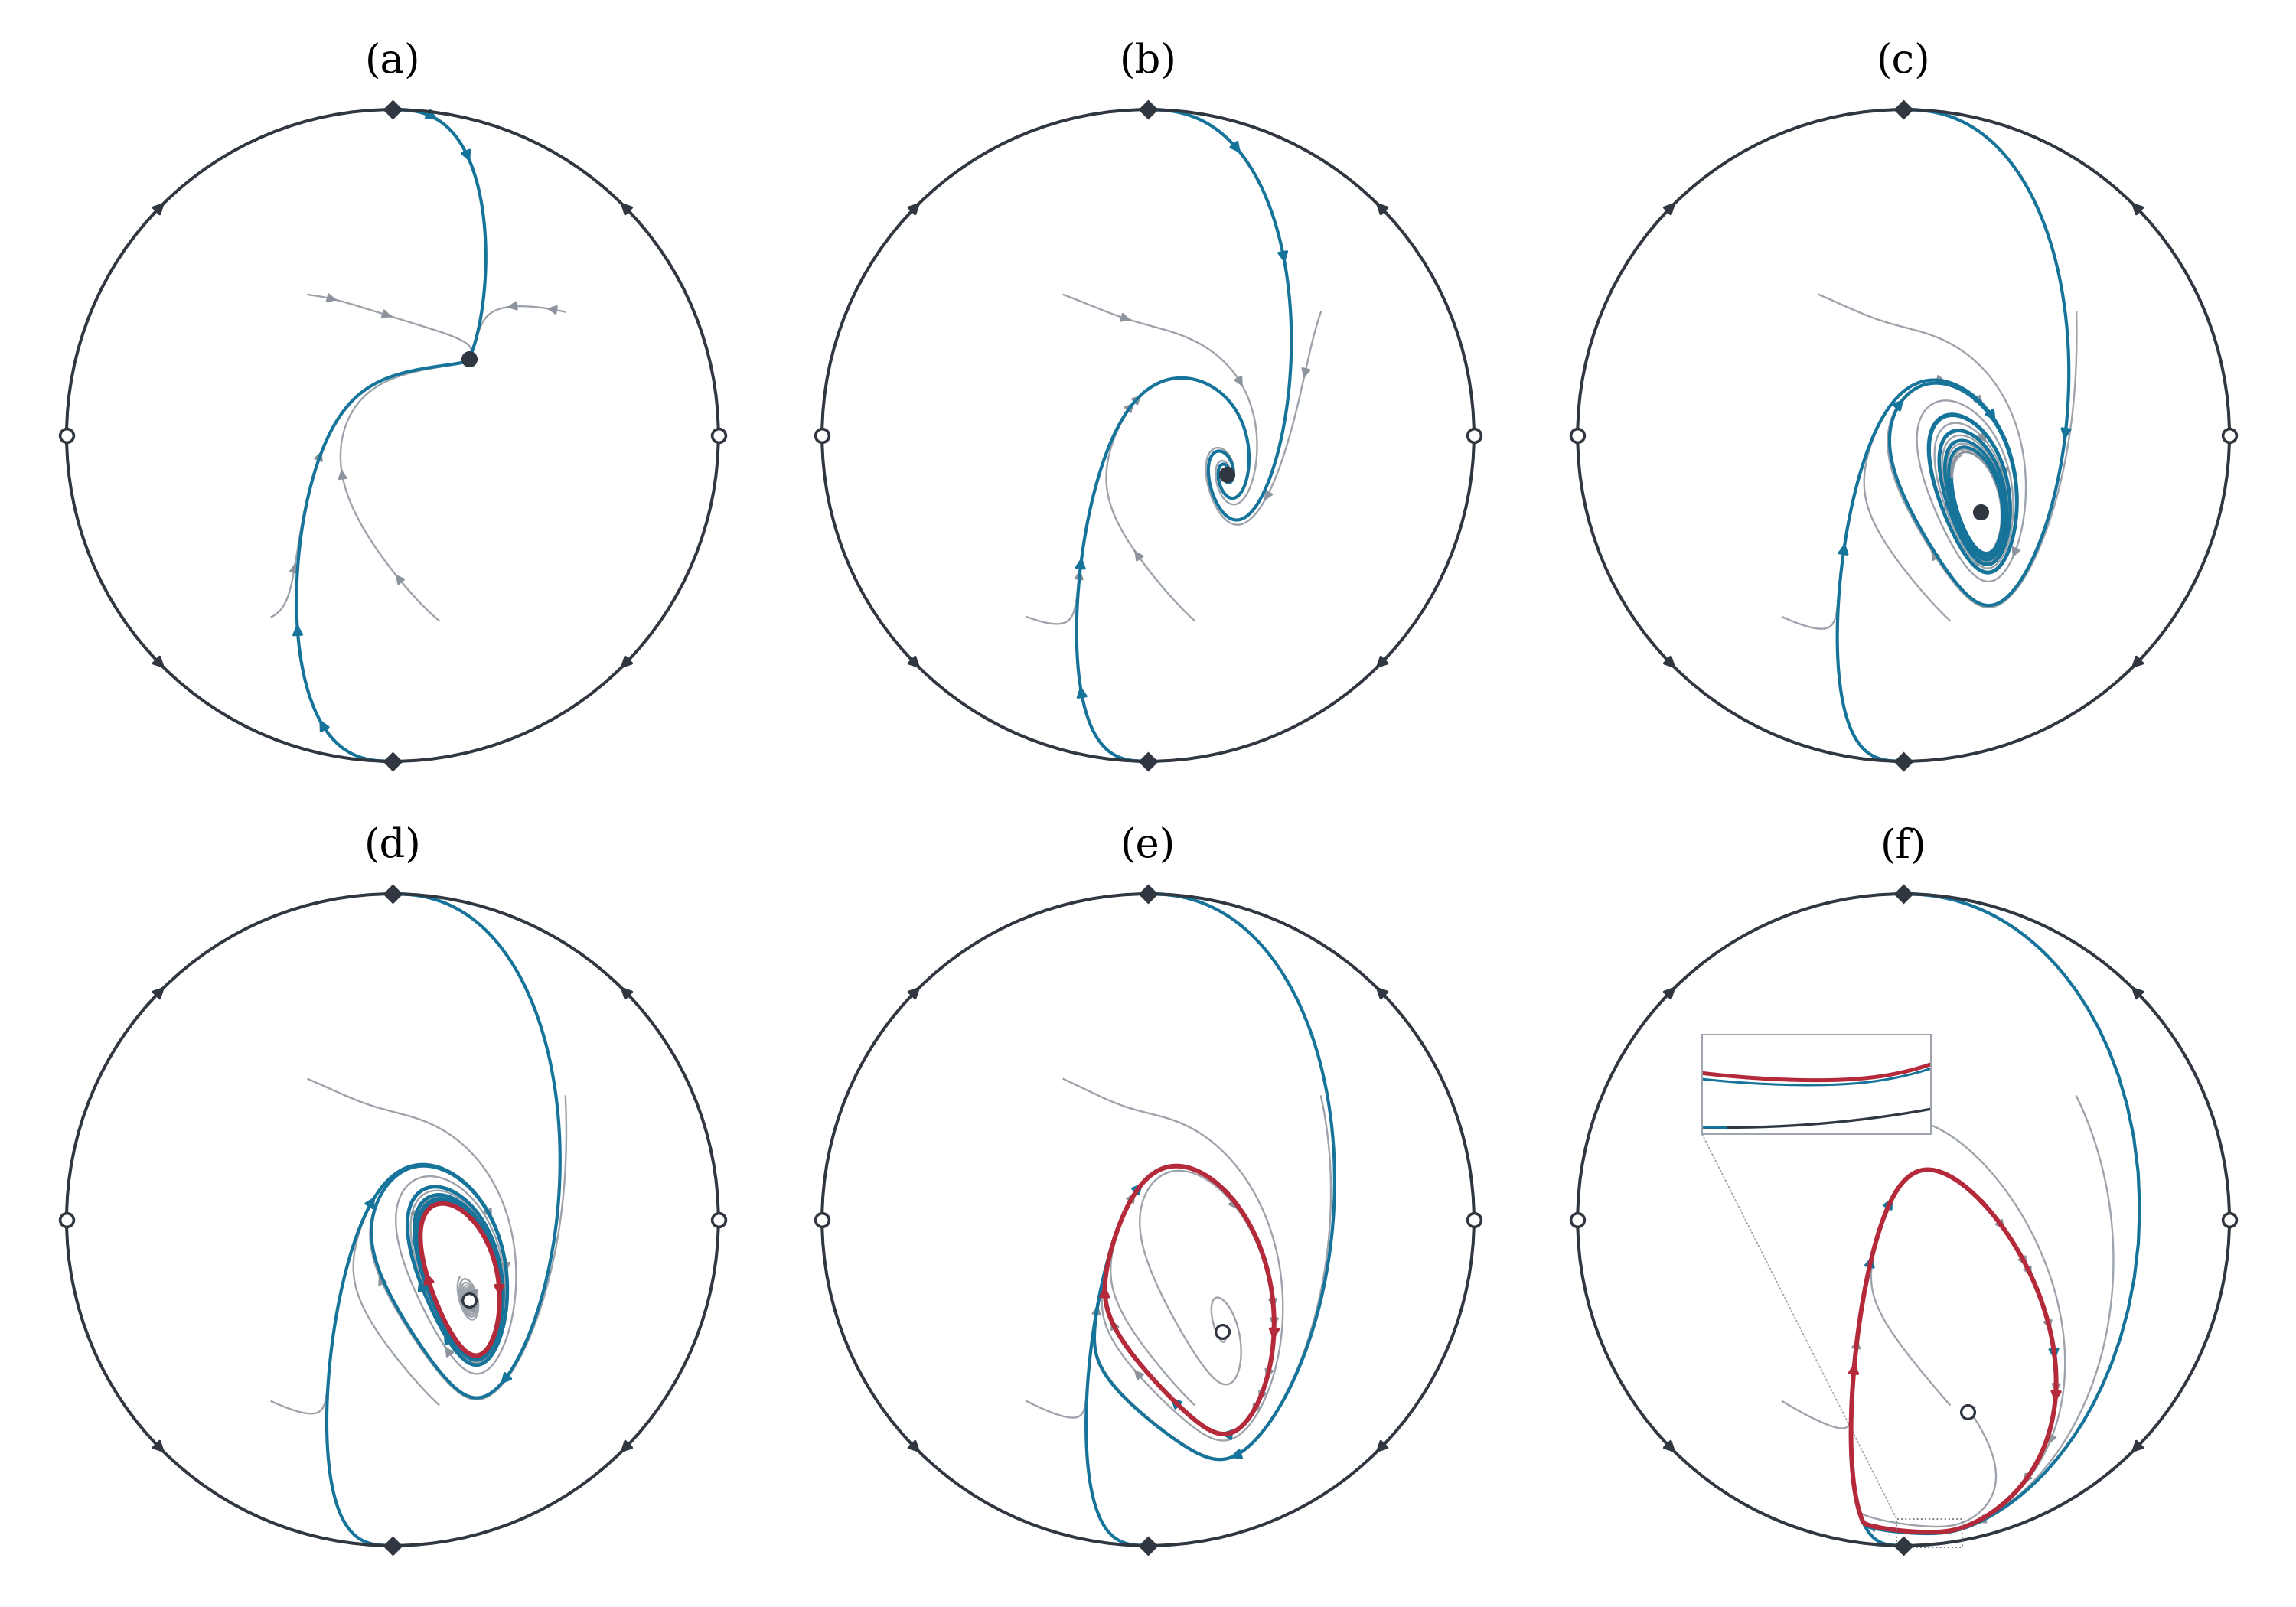
\includegraphics[width=\linewidth]{HR}
    \caption{Panels (a)--(f) correspond, respectively, to
    $k=0$, $1.5$, $2$, $2.05$, $2.5$, and $4$; the Hopf value
    is $k_H=2$.
    The finite equilibrium $E_*=(1,1-k)$ is a stable node
    in (a), a stable focus in (b), a stable weak focus in (c),
    an unstable focus in (d)--(e), and an unstable node in (f).
    Filled and open circles denote attracting and repelling
    equilibria, respectively.
    The two horizontal boundary points are source nodes,
    whereas the vertical diamonds denote degenerate boundary
    saddles, each with two incoming boundary separatrices,
    one outgoing interior separatrix, and two hyperbolic
    sectors on the disk side.
    Blue curves are numerical approximations of the outgoing
    interior separatrices from infinity; gray curves are
    sample trajectories, and arrows indicate forward time.
    Red curves in (d)--(f) are numerically computed attracting
    periodic orbits; panel (d) illustrates a parameter value
    near the Hopf threshold.
    The inset in (f) magnifies the indicated lower-boundary
    region and distinguishes the periodic orbit from the
    blue separatrix and the disk boundary.
    The interior trajectories were obtained by direct
    numerical integration.
    }
    \label{fig:hr-representative-portraits}
\end{figure}




















%\section*{Acknowledgments}
%[Funding, collaborations]

\bibliographystyle{plain}
\bibliography{bibliography}
%\printbibliography




\end{document}
